\chapter{Independent Sets, Cliques, and Vertex Covers}

In the preceding chapter, we saw that coloring a graph partitions its vertices into
conflict-free subsets. Each color class is an independent set. Naturally, this leads
to an optimization question: how large can a single conflict-free set be?
Three fundamental optimization problems on a graph turn out to be direct translations
of one another. Pick a graph. What is the largest set of
vertices with \emph{no} edge between any two of them? What is the largest set of
vertices with \emph{every} edge present between them? And what is the smallest set
of vertices that \emph{touches} every edge? The first is the \emph{independent set},
the second the \emph{clique}, the third the \emph{vertex cover}. A solution to
any one of them gives, with two lines of reasoning, solutions to all three.

These three problems are among the most basic NP-hard problems on graphs.
There is no flow trick, no augmenting path, no spanning-tree exchange that finds a
maximum clique in polynomial time. But vertex cover admits three algorithmic
approaches: a factor-$2$ approximation, a half-integral linear programming relaxation,
and a fixed-parameter tractable branch-and-bound algorithm when the cover is small.
Here we examine all three tools on this shared foundation.

\begin{historybox}
The trio of independent set, clique, and vertex cover represents the historical core of
combinatorial optimization. In 1959, Hungarian mathematician Tibor Gallai established the
fundamental identities $\alpha(\Gph) + \tau(\Gph) = n$ and $\alpha'(\Gph) + \tau'(\Gph) = n$,
proving that maximum independent sets and minimum vertex covers are algebraic complements.
In 1972, Richard Karp included all three problems in his foundational list of 21 NP-complete
problems, proving that exact polynomial-time optimization is intractable in general.

Early heuristics attempted greedy degree-based selection, but such choices can get trapped
in small sub-optimal sets. In 1965, J.W. Moon and Leo Moser proved that an $n$-vertex graph
can contain up to $3^{n/3} \approx 1.442^n$ maximal cliques. In 1973, Coenraad Bron and Joep
Kerbosch introduced their classic recursive backtracking algorithm with a pivot rule that
avoids redundant searches and matches the Moon--Moser worst-case bound.

Approximation and linear programming opened a new chapter. In the 1970s, Fanica Gavril and
Mihalis Yannakakis observed that a maximal matching immediately yields a 2-approximation for
vertex cover by taking both endpoints of each matched edge. George Nemhauser and Leslie
Trotter (1975) proved that the standard LP relaxation is half-integral: every variable takes
value in $\{0, \tfrac{1}{2}, 1\}$, and variables assigned integer values are guaranteed to
agree with some optimal integer solution, providing an exact kernelization reduction.
Whether vertex cover can be approximated within $2-\eps$ remains a major open problem,
conjectured to be NP-hard under Subhash Khot's Unique Games Conjecture (2002).
\end{historybox}

\chapterline

\section{Three Problems and Their Complements}
\label{ch29:trinity}

Fix a simple undirected graph $\Gph=(V,E)$ with $n=\abs{V}$ vertices and
$m=\abs{E}$ edges. We need three definitions, and then one picture ties them
together for the rest of the chapter.

\begin{definition}[Independent set]
\label{ch29:def-is}
A set $S\subseteq V$ is \emph{independent} (or \emph{stable}) if no edge of
$\Gph$ has both endpoints in $S$: for all $u,v\in S$, $\set{u,v}\notin E$. The
\emph{independence number} $\alpha(\Gph)$ is the size of a largest independent
set.
\end{definition}

\begin{definition}[Clique]
\label{ch29:def-clique}
A set $K\subseteq V$ is a \emph{clique} if every pair of its vertices is joined
by an edge: for all distinct $u,v\in K$, $\set{u,v}\in E$. The \emph{clique
number} $\omega(\Gph)$ is the size of a largest clique.
\end{definition}

\begin{definition}[Vertex cover]
\label{ch29:def-vc}
A set $C\subseteq V$ is a \emph{vertex cover} if every edge has at least one
endpoint in $C$: for all $\set{u,v}\in E$, $u\in C$ or $v\in C$. The \emph{vertex
cover number} $\tau(\Gph)$ is the size of a smallest vertex cover.
\end{definition}

\begin{intuitionbox}
Read the three definitions as three sentences about edges. An independent set
says ``no edge lives inside me.'' A clique says ``every possible edge lives
inside me.'' A vertex cover says ``no edge escapes me.'' The first and third are
about the \emph{same} edges: if $S$ contains no edge, then every edge must have
an endpoint outside $S$, i.e. in the complement $V\setminus S$. This observation
is the Gallai identity below.
\end{intuitionbox}

Here is the running graph for the chapter. Call it $\Gph_0$
(Figure~\ref{ch29:fig-g0}): six vertices, drawn so that the three structures are
visible at a glance.

\begin{figure}[H]
\centering
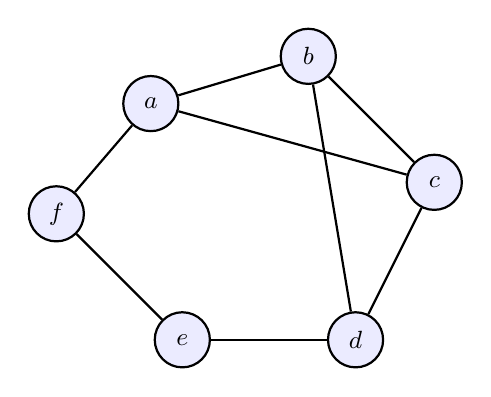
\begin{tikzpicture}[every node/.style={circle,draw,fill=blue!8,minimum size=7mm,
   font=\small,inner sep=0pt},thick]
  \node (a) at (0,2)   {$a$};
  \node (b) at (2,2.6) {$b$};
  \node (c) at (3.6,1) {$c$};
  \node (d) at (2.6,-1){$d$};
  \node (e) at (0.4,-1){$e$};
  \node (f) at (-1.2,0.6){$f$};
  \draw (a)--(b); \draw (b)--(c); \draw (a)--(c);
  \draw (c)--(d); \draw (b)--(d);
  \draw (d)--(e); \draw (e)--(f); \draw (a)--(f);
\end{tikzpicture}
\caption{The running graph $\Gph_0$ with eight edges. The triangles $\set{a,b,c}$
and $\set{b,c,d}$ are its cliques of size $3$; the path $f\,e\,d$ and the pendant
edges $af,de,ef$ hang off them.}
\label{ch29:fig-g0}
\end{figure}

The triangle $\set{a,b,c}$ is a clique of size $3$. The set $\set{a,d}$ is
independent (no edge between them), and so is $\set{b,e}$. Let us not give away
all the answers yet; we trace them by hand in Section~\ref{ch29:bk-trace}. First,
we relate the three problems.

\subsection{Independent set $=$ clique in the complement}

\begin{definition}[Complement graph]
\label{ch29:def-complement}
The \emph{complement} $\overline{\Gph}=(V,\overline{E})$ has the same vertices
and exactly the non-edges of $\Gph$: $\set{u,v}\in\overline{E}$ if and only if
$u\neq v$ and $\set{u,v}\notin E$.
\end{definition}

\begin{proposition}[Independent--clique duality]
\label{ch29:prop-is-clique}
A set $S\subseteq V$ is independent in $\Gph$ if and only if $S$ is a clique in
$\overline{\Gph}$. Consequently $\alpha(\Gph)=\omega(\overline{\Gph})$ and
$\omega(\Gph)=\alpha(\overline{\Gph})$.
\end{proposition}

\begin{proof}
$S$ independent in $\Gph$ means no pair inside $S$ is an edge of $\Gph$, i.e.
every pair inside $S$ is a non-edge of $\Gph$, i.e. every pair inside $S$ is an
edge of $\overline{\Gph}$ -- which is exactly the statement that $S$ is a clique
in $\overline{\Gph}$. The numerical identities follow by taking the largest such
$S$, and the second comes from $\overline{\overline{\Gph}}=\Gph$.
\end{proof}

This duality has \emph{algorithmic} consequences.
Any algorithm for maximum clique runs unchanged as a maximum independent set
algorithm on the complement, and vice versa. The Bron--Kerbosch enumeration we
build in Section~\ref{ch29:bron-kerbosch} is universally phrased for cliques;
feed it $\overline{\Gph}$ and it lists maximal independent sets. The only cost is
that complementation flips edge density: a sparse $\Gph$ has a dense
$\overline{\Gph}$, which matters for the running time but never for correctness.

\subsection{Gallai: cover and independent set partition the vertices}

\begin{theorem}[Gallai's identity]
\label{ch29:thm-gallai}
$S\subseteq V$ is independent in $\Gph$ if and only if its complement
$C=V\setminus S$ is a vertex cover. Hence for every graph on $n$ vertices,
\[
  \alpha(\Gph)+\tau(\Gph)=n .
\]
\end{theorem}

\begin{proof}
Suppose $S$ is independent. Take any edge $\set{u,v}\in E$. Since $S$ contains no
edge, $u$ and $v$ are not both in $S$, so at least one lies in $C=V\setminus S$.
Thus $C$ covers every edge: $C$ is a vertex cover. Conversely, suppose $C$ is a
vertex cover and let $S=V\setminus C$. If some edge $\set{u,v}$ had both
endpoints in $S$, then \emph{neither} endpoint is in $C$, contradicting that $C$
covers $\set{u,v}$. So $S$ is independent.

The map $S\mapsto V\setminus S$ is a bijection between independent sets and
vertex covers that sends a set of size $k$ to a set of size $n-k$. A largest
independent set therefore corresponds to a smallest vertex cover, giving
$\alpha(\Gph)=n-\tau(\Gph)$ (Figure~\ref{ch29:fig-trinity-duality}).
\end{proof}

\begin{figure}[H]
\centering
\begin{tikzpicture}[>=Stealth, every node/.style={font=\small},
  vnode/.style={circle,draw=nodeblue,fill=blue!8,thick,minimum size=6.5mm,inner sep=0pt,font=\footnotesize},
  isnode/.style={circle,draw=targetgreen,fill=targetgreen!20,very thick,minimum size=6.5mm,inner sep=0pt,font=\footnotesize\bfseries},
  vcnode/.style={circle,draw=trapred,fill=trapred!18,very thick,minimum size=6.5mm,inner sep=0pt,font=\footnotesize\bfseries},
  clnode/.style={circle,draw=structurepurple,fill=structurepurple!20,very thick,minimum size=6.5mm,inner sep=0pt,font=\footnotesize\bfseries}
]
  % Left panel: Gallai partition on G_0
  \begin{scope}[xshift=-3.6cm]
    \node[font=\footnotesize\bfseries,text=sourceblue!85!black] at (1.3,3.3) {Gallai Partition on $\Gph_0$: $V = S \sqcup C$};
    \node[isnode] (a1) at (0,2.0)   {$a$};
    \node[vcnode] (b1) at (1.6,2.4) {$b$};
    \node[vcnode] (c1) at (2.8,1.0) {$c$};
    \node[isnode] (d1) at (2.0,-0.6){$d$};
    \node[vcnode] (e1) at (0.3,-0.6){$e$};
    \node[vcnode] (f1) at (-0.8,0.8){$f$};
    \draw[thick,edgegray] (a1)--(b1) (b1)--(c1) (a1)--(c1) (c1)--(d1) (b1)--(d1) (d1)--(e1) (e1)--(f1) (a1)--(f1);
    \node[font=\scriptsize,align=center] at (1.0,-1.45) {\textcolor{targetgreen!80!black}{\textbf{Indep.\ set}} $S=\{a,d\}$ ($\alpha=2$)\\[-1pt]\textcolor{trapred!85!black}{\textbf{Vertex cover}} $C=V\setminus S=\{b,c,e,f\}$ ($\tau=4$)};
  \end{scope}

  % Divider
  \draw[gray!35,dashed] (0,-1.8) -- (0,3.5);

  % Right panel: Complement graph bar(G_0)
  \begin{scope}[xshift=2.3cm]
    \node[font=\footnotesize\bfseries,text=structurepurple!85!black] at (1.3,3.3) {Complement $\overline{\Gph_0}$: $S$ Becomes a Clique};
    \node[clnode] (a2) at (0,2.0)   {$a$};
    \node[vnode]  (b2) at (1.6,2.4) {$b$};
    \node[vnode]  (c2) at (2.8,1.0) {$c$};
    \node[clnode] (d2) at (2.0,-0.6){$d$};
    \node[vnode]  (e2) at (0.3,-0.6){$e$};
    \node[vnode]  (f2) at (-0.8,0.8){$f$};
    \draw[thick,gray!55] (a2)--(e2) (b2)--(e2) (b2)--(f2) (c2)--(e2) (c2)--(f2) (d2)--(f2);
    \draw[very thick,structurepurple] (a2)--(d2);
    \node[font=\scriptsize,align=center] at (1.0,-1.45) {Non-edge $ad \notin E(\Gph_0)$ becomes edge $ad \in E(\overline{\Gph_0})$\\[-1pt]\textcolor{structurepurple!85!black}{\textbf{Max clique}} $\{a,d\}$ in $\overline{\Gph_0}$ ($\omega(\overline{\Gph_0})=\alpha(\Gph_0)=2$)};
  \end{scope}
\end{tikzpicture}
\caption{The two structural relationships on $\Gph_0$. \textbf{Left (Gallai):} Every edge of $\Gph_0$ has at least one red endpoint in the cover $C=\{b,c,e,f\}$, leaving the green independent set $S=\{a,d\}$ completely edge-free ($\alpha+\tau=2+4=6$). \textbf{Right (Complement):} Flipping edges and non-edges turns the independent set $S=\{a,d\}$ of $\Gph_0$ into a clique in $\overline{\Gph_0}$.}
\label{ch29:fig-trinity-duality}
\end{figure}

\begin{focusbox}
Three numbers, one identity each, all on $\Gph_0$:
\[
   \alpha(\Gph_0)+\tau(\Gph_0)=6,\qquad
   \alpha(\Gph_0)=\omega(\overline{\Gph_0}),\qquad
   \omega(\Gph_0)=\alpha(\overline{\Gph_0}).
\]
The first is Gallai (complement \emph{within} $\Gph_0$); the second and third are
the complement-graph duality (a \emph{different} graph). Do not conflate ``the
complement of a set'' with ``the complement of a graph.'' Gallai uses the former,
Proposition~\ref{ch29:prop-is-clique} the latter.
\end{focusbox}

\begin{trapbox}
Gallai's $\alpha+\tau=n$ is exact and holds for \emph{every} graph -- it is a
genuine equation, not an inequality or an approximation. The temptation is to
expect a parallel identity tying $\omega$ to the other two. There is none of the
same simplicity: $\omega$ relates to the rest only through the complement graph,
where $\omega(\Gph)=\alpha(\overline{\Gph})=n-\tau(\overline{\Gph})$. So clique
size is a statement about $\overline{\Gph}$'s cover, not $\Gph$'s. Mixing these
up produces ``identities'' that are false on the very first triangle you test.
\end{trapbox}

\begin{connectionbox}
On \emph{bipartite} graphs these three problems become tractable.
K\"onig's theorem (Chapter~15) says $\tau(\Gph)=\nu(\Gph)$,
the size of a maximum matching, whenever $\Gph$ is bipartite. Through Gallai,
$\alpha(\Gph)=n-\nu(\Gph)$, so maximum independent set on bipartite graphs is
just maximum matching -- solvable by augmenting paths in polynomial time. The
hardness we meet below is therefore a non-bipartite, odd-cycle phenomenon, the
same obstruction that forced Edmonds to invent blossoms for general matching.
\end{connectionbox}

\section{Enumerating Cliques: Bron--Kerbosch}
\label{ch29:bron-kerbosch}

Finding one maximum clique is NP-hard (Section~\ref{ch29:hardness}). But many
applications -- community detection, computational chemistry, the analysis of
social networks -- want \emph{all} maximal cliques, and there a simple
recursion does the job. The Bron--Kerbosch algorithm enumerates every maximal
clique exactly once, and on real instances it is fast despite the worst case
being unavoidable (a graph can have $3^{n/3}$ maximal cliques, and you cannot
list them in less time than it takes to write them down).

\begin{definition}[Maximal vs.\ maximum]
\label{ch29:def-maximal}
A clique is \emph{maximal} if no vertex can be added to it while keeping it a
clique. It is \emph{maximum} if it is the largest clique in the graph. Maximum
implies maximal; the converse fails -- a maximal clique can be small if it is
``stuck.''
\end{definition}

\begin{intuitionbox}
The recursion grows a clique vertex by vertex. It keeps three sets: $R$, the
vertices already committed to the current clique; $P$, the candidates that are
adjacent to all of $R$ and could still extend it; and $X$, vertices that are also
adjacent to all of $R$ but have \emph{already} been used as the start of some
branch. When both $P$ and $X$ are empty, $R$ cannot be extended by anyone -- it
is maximal, and we report it. $X$ is the bookkeeping that prevents the same
maximal clique from being printed twice: it remembers ``we already explored that
direction.''
\end{intuitionbox}

\begin{algorithm}[H]
\caption{\textsc{BronKerbosch}$(R,P,X)$ -- enumerate maximal cliques}
\label{ch29:alg-bk}
\DontPrintSemicolon
\SetKwInOut{Input}{input}\SetKwInOut{Output}{output}
\Input{committed set $R$, candidates $P$, excluded $X$; initial call $(\emptyset,V,\emptyset)$}
\Output{every maximal clique, each printed once}
\If{$P=\emptyset$ \textbf{and} $X=\emptyset$}{
  report $R$ as a maximal clique\;
  \Return\;
}
choose a \emph{pivot} $u\in P\cup X$ maximizing $\abs{P\cap N(u)}$\;
\ForEach{$v\in P\setminus N(u)$}{
  \textsc{BronKerbosch}$\bigl(R\cup\set{v},\; P\cap N(v),\; X\cap N(v)\bigr)$\;
  $P\leftarrow P\setminus\set{v}$\;
  $X\leftarrow X\cup\set{v}$\;
}
\end{algorithm}

Here $N(u)$ is the open neighborhood of $u$. The recursion branches on $v$, moves
$v$ into the committed set $R$, and restricts the candidate and excluded sets to
$v$'s neighbors -- because any clique containing $R\cup\set v$ can only use
vertices adjacent to $v$. After exploring the branch through $v$, we retire $v$
from $P$ into $X$: future branches must avoid $v$, or they would re-list cliques
already found.

\subsection{The Pivot: Pruning Redundant Search Branches}
\label{ch29:bk-pivot}

The naive version omits the pivot and simply loops over all $v\in P$. It is
correct but slow, because it explores branches that cannot possibly yield a
\emph{new} maximal clique. The pivot fixes this.

\begin{whybox}
Fix any maximal clique $K\supseteq R$ that we still hope to find from $(R,P,X)$.
Let $u\in P\cup X$ be the pivot. Either $u\in K$, or some non-neighbor of $u$ is
in $K$ -- because $K$ is maximal, so if $u$ itself were addable it would be
forced in, meaning $K$ must contain a vertex that blocks $u$, i.e. a non-neighbor
of $u$. In both cases $K$ contains a vertex of $\set{u}\cup(P\setminus N(u))$.
The branches we actually take are exactly $P\setminus N(u)$ (and the pivot's own
fate is handled because $u$ stays available in those sub-branches). So looping
over $P\setminus N(u)$ misses nothing: every maximal clique reachable from here
passes through one of these branches. Choosing $u$ to \emph{maximize}
$\abs{P\cap N(u)}$ makes $P\setminus N(u)$ as small as possible -- the fewest
branches.
\end{whybox}

\begin{figure}[H]
\centering
\begin{tikzpicture}[>=Stealth,
  statebox/.style={rounded corners=3pt,thick,inner sep=6pt,font=\footnotesize},
  vnode/.style={circle,draw,thick,minimum size=6mm,inner sep=0pt,font=\scriptsize}
]
  % Lane 1: Partition (R, P, X)
  \node[font=\footnotesize\bfseries\scshape,text=sourceblue!80!black,anchor=west] at (-5.8,2.4) {Lane 1: Recursive State Partition $(R, P, X)$};
  \draw[gray!30,dashed] (-5.8,2.2) -- (5.8,2.2);

  \node[statebox,draw=targetgreen,fill=targetgreen!12,text width=30mm,align=center] (Rbox) at (-4.1,1.4) {
    \textbf{Committed Set $R$}\\[2pt]
    Clique so far\\(all pairs adjacent)
  };
  \node[statebox,draw=sourceblue,fill=sourceblue!12,text width=38mm,align=center] (Pbox) at (0.0,1.4) {
    \textbf{Candidate Set $P$}\\[2pt]
    Common neighbors of $R$\\not yet branched on
  };
  \node[statebox,draw=trapred,fill=trapred!12,text width=30mm,align=center] (Xbox) at (4.1,1.4) {
    \textbf{Excluded Set $X$}\\[2pt]
    Common neighbors\\already retired
  };

  % Transition arrow
  \draw[->,very thick,structurepurple] (0,0.6) -- (0,0.0) node[midway,right=2pt,font=\scriptsize\bfseries] {choose pivot $u \in P \cup X$};

  % Lane 2: The Pivot Pruning
  \node[font=\footnotesize\bfseries\scshape,text=structurepurple!80!black,anchor=west] at (-5.8,-0.2) {Lane 2: Branching Selection via Pivot $u$};
  \draw[gray!30,dashed] (-5.8,-0.4) -- (5.8,-0.4);

  % Sub-boxes inside P
  \node[rounded corners=2pt,draw=edgegray,fill=gray!15,dashed,text width=42mm,minimum height=14mm,align=center] (pruned) at (-2.4,-1.4) {
    \textbf{Pruned Neighbors}\\[2pt]
    $P \cap N(u)$\\[1pt]
    {\tiny (No need to branch: covered by $u$)}
  };
  \node[rounded corners=2pt,draw=sourceblue,fill=sourceblue!20,thick,text width=42mm,minimum height=14mm,align=center] (active) at (2.4,-1.4) {
    \textbf{Active Branches}\\[2pt]
    $v \in P \setminus N(u)$\\[1pt]
    {\tiny (Branch on $v$, then retire $v$ to $X$)}
  };

  \draw[<->,thick,edgegray] (-4.6,-2.4) -- (4.6,-2.4) node[midway,below=2pt,font=\scriptsize] {Full candidate pool $P$};
\end{tikzpicture}
\caption{The Bron--Kerbosch state partition and pivot optimization. \textbf{Top (Lane~1):} The vertex set is divided into committed clique vertices $R$, candidates $P$ adjacent to all of $R$, and already-explored vertices $X$. \textbf{Bottom (Lane~2):} Selecting a pivot $u$ maximizing $|P\cap N(u)|$ proves that every maximal clique containing $R$ either contains $u$ or a non-neighbor of $u$. The algorithm branches only on the restricted set $v \in P \setminus N(u)$, pruning all neighbors of $u$ from branching and drastically collapsing the search tree.}
\label{ch29:fig-bk-pivot}
\end{figure}

\begin{lemma}[Correctness of Bron--Kerbosch]
\label{ch29:lem-bk-correct}
Algorithm~\ref{ch29:alg-bk} reports a set $R$ if and only if $R$ is a maximal
clique, and reports each maximal clique exactly once.
\end{lemma}

\begin{proof}
\emph{Invariant.} At every call $(R,P,X)$, the set $R$ is a clique, and
$P\cup X$ is exactly the set of vertices adjacent to every vertex of $R$ (the
common neighborhood). $P$ holds those not yet branched on at an ancestor; $X$
holds those already retired. This holds at the root $(\emptyset,V,\emptyset)$ and
is preserved by the recursion, since restricting to $N(v)$ keeps precisely the
common neighbors of $R\cup\set v$, and the moves $P\to X$ respect the split.

\emph{Reports only maximal cliques.} When $P=X=\emptyset$, no vertex is adjacent
to all of $R$, so $R$ cannot be extended: it is maximal.

\emph{Reports every maximal clique once.} Let $K$ be maximal. Existence of a
branch that builds it follows from the pivot argument above: at each level a
vertex of $K$ lies in the looped set $P\setminus N(u)$, so the recursion can
descend into $K$, committing its vertices one at a time until $P=X=\emptyset$ and
$R=K$. Uniqueness follows from $X$: once a vertex $v$ is retired into $X$, every
descendant call carries $v$ in its $X$ component whenever $v$ is a common
neighbor, so the maximality test $X=\emptyset$ forbids re-reporting any clique
that could have included $v$ earlier. Hence each maximal clique is emitted in
exactly one leaf.
\end{proof}

\subsection{Tracing it on $\Gph_0$}
\label{ch29:bk-trace}

Take the running graph. The adjacency lists are
\[
\begin{aligned}
&N(a)=\set{b,c,f}, &&N(b)=\set{a,c,d}, &&N(c)=\set{a,b,d},\\
&N(d)=\set{b,c,e}, &&N(e)=\set{d,f},   &&N(f)=\set{a,e}.
\end{aligned}
\]
Start with $R=\emptyset$, $P=\set{a,b,c,d,e,f}$, $X=\emptyset$. Pick a pivot in
$P\cup X$ maximizing $\abs{P\cap N(u)}$: vertices $a,b,c,d$ each have degree $3$,
so any of them ties; take $u=c$, giving $P\cap N(c)=\set{a,b,d}$ and a loop over
$P\setminus N(c)=\set{c,e,f}$ (note $c$ itself is a non-neighbor of itself under
the open-neighborhood convention, so it appears in the loop). The loop processes
$c$, then $e$, then $f$, retiring each into $X$ as it goes.

The table below follows the recursion in execution order, one row per call. The
\emph{depth} column tracks how deep in the recursion the call sits; the
\emph{pivot, loop} column shows the pivot chosen at that call and the resulting
loop set; a leaf with empty $P$ and $X$ reports the clique $R$.

\begin{center}
\renewcommand{\arraystretch}{1.25}
\begin{tabular}{@{}lllll@{}}
\toprule
depth & $v$ & call $(R;P;X)$ & pivot, loop & event \\
\midrule
0 & --   & $(\emptyset;\,abcdef;\,\emptyset)$ & $c$, loop $\set{c,e,f}$ & \\
1 & $c$  & $(c;\,abd;\,\emptyset)$            & $b$, loop $\set{b}$     & \\
2 & $b$  & $(bc;\,ad;\,\emptyset)$            & $a$, loop $\set{a,d}$   & \\
3 & $a$  & $(abc;\,\emptyset;\,\emptyset)$    & --                      & \textbf{report }$\set{a,b,c}$\\
3 & $d$  & $(bcd;\,\emptyset;\,\emptyset)$    & --                      & \textbf{report }$\set{b,c,d}$\\
1 & $e$  & $(e;\,df;\,\emptyset)$             & $d$, loop $\set{d,f}$   & \\
2 & $d$  & $(de;\,\emptyset;\,\emptyset)$     & --                      & \textbf{report }$\set{d,e}$\\
2 & $f$  & $(ef;\,\emptyset;\,\emptyset)$     & --                      & \textbf{report }$\set{e,f}$\\
1 & $f$  & $(f;\,a;\,e)$                      & $a$, loop $\set{a}$      & \\
2 & $a$  & $(af;\,\emptyset;\,\emptyset)$     & --                      & \textbf{report }$\set{a,f}$\\
\bottomrule
\end{tabular}
\end{center}

So the full census of maximal cliques of $\Gph_0$ is
\[
  \set{a,b,c},\quad \set{b,c,d},\quad \set{d,e},\quad \set{e,f},\quad \set{a,f},
\]
five in all, each reported once. The triangles $\set{a,b,c}$ and $\set{b,c,d}$ are
the two maximum cliques, so $\omega(\Gph_0)=3$. Note the effect of the pivot. At
the root, choosing $c$ keeps only the three branches $\set{c,e,f}$ instead of all
six vertices; both triangles then fall out of the single $c$-branch, because once
$c$ is committed the candidate set $\set{a,b,d}$ already contains everything the
triangles need. The excluded set $X$ prevents duplicate cliques in the last branch: the call
$(f;\,a;\,e)$ carries $e$ in $X$ because $e$ is a common neighbor of $f$ already
explored through the $e$-rooted branch, so the clique $\set{e,f}$ found there is
not reported a second time from underneath $f$.

The complement $\overline{\Gph_0}$ makes the independent-set side visible. Its
edges are exactly the seven non-edges of $\Gph_0$, and a maximal clique of
$\overline{\Gph_0}$ is a maximal independent set of $\Gph_0$
(Proposition~\ref{ch29:prop-is-clique}). Drawn below, $\overline{\Gph_0}$ has no
triangle, so its largest clique -- and hence $\alpha(\Gph_0)$ -- is just $2$.

\begin{figure}[H]
\centering
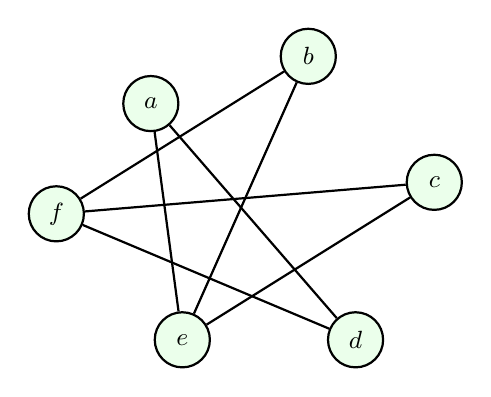
\begin{tikzpicture}[every node/.style={circle,draw,fill=green!8,minimum size=7mm,
   font=\small,inner sep=0pt},thick]
  \node (a) at (0,2)   {$a$};
  \node (b) at (2,2.6) {$b$};
  \node (c) at (3.6,1) {$c$};
  \node (d) at (2.6,-1){$d$};
  \node (e) at (0.4,-1){$e$};
  \node (f) at (-1.2,0.6){$f$};
  % non-edges of G_0: a-d, a-e, b-e, b-f, c-e, c-f, d-f
  \draw (a)--(d); \draw (a)--(e); \draw (b)--(e);
  \draw (b)--(f); \draw (c)--(e); \draw (c)--(f); \draw (d)--(f);
\end{tikzpicture}
\caption{The complement $\overline{\Gph_0}$: its seven edges are the non-edges of
$\Gph_0$. It is triangle-free, so $\omega(\overline{\Gph_0})=\alpha(\Gph_0)=2$.}
\label{ch29:fig-complement}
\end{figure}

\begin{labbox}
Re-run the recursion yourself, this time choosing a different root pivot among the
degree-$3$ vertices (say $a$ instead of $c$) and confirm you still recover exactly
the five cliques above with no repeats -- $X$ is precisely what suppresses
those duplicates. Then take the complement
$\overline{\Gph_0}$ of Figure~\ref{ch29:fig-complement} and re-run Bron--Kerbosch
on it: the maximal cliques you find are the maximal
\emph{independent sets} of $\Gph_0$. You should find that every maximal
independent set has size $2$ -- for instance $\set{a,d}$ and $\set{a,e}$ both fail
to extend -- so $\alpha(\Gph_0)=2$. Which vertex blocks each attempt to grow
$\set{a,e}$ to size three?
\end{labbox}

\subsection{Complexity}

\begin{theorem}[Tomita--Tanaka--Takahashi bound]
\label{ch29:thm-bk-time}
With pivoting, Bron--Kerbosch runs in $\Oh(3^{n/3})$ time.
\end{theorem}

\begin{proof}[Idea]
The number of leaves of the recursion tree is bounded by the number of maximal
cliques, and Moon and Moser proved a graph on $n$ vertices has at most $3^{n/3}$
maximal cliques (a disjoint union of triangles achieves it). The pivot guarantees
each internal node's branching factor is controlled so that the total work is
within a polynomial factor of the leaf count, and a careful accounting collapses
that to $\Oh(3^{n/3})$ overall.
\end{proof}

\begin{complexitybox}
\textbf{Bron--Kerbosch with pivot.} Worst-case time $\Oh(3^{n/3})$, optimal in
the output-size sense (you cannot beat the number of cliques you must print).
Memory is $\Oh(n^2)$ for the adjacency structure plus $\Oh(n)$ recursion depth
times the set representations. A degeneracy-ordering variant achieves
$\Oh(d\,n\,3^{d/3})$ where $d$ is the graph's \emph{degeneracy}, near-linear in
$n$ for sparse graphs of small degeneracy -- the version used in practice on
large social networks. Representing $P,X$ as bitsets gives a constant-factor gain that
matters a great deal in practice.
\end{complexitybox}

\begin{applicationbox}
Bron--Kerbosch is the standard algorithm behind clique-based community detection,
protein--protein interaction analysis, and the ``maximum common subgraph''
matching used in cheminformatics (mapping one molecule's structure onto
another's reduces to finding large cliques in a product graph). The
degeneracy-ordered variant of Eppstein, L\"offler, and Strash (2010) is what lets
it scale to graphs with millions of edges.
\end{applicationbox}

\section{Vertex Cover: The LP Relaxation and Half-Integrality}
\label{ch29:lp}

Vertex cover is the most tractable of the three, because of a linear
program with a useful property: its optimal solutions can always be taken
to use only the values $0$, $\tfrac12$, and $1$. This half-integrality
underlies both the $2$-approximation and the parameterized algorithm, so we
build it carefully.

Assign a variable $x_v\in\set{0,1}$ to each vertex, meaning ``$v$ is in the
cover.'' The covering requirement -- every edge has an endpoint in $C$ -- is
$x_u+x_v\ge 1$ for each edge $\set{u,v}$. Minimizing the size of the cover is
minimizing $\sum_v x_v$. So the exact problem is the integer program

\begin{equation}
\label{ch29:ip}
\tau(\Gph)\;=\;\min\ \sum_{v\in V} x_v
  \quad\text{s.t.}\quad x_u+x_v\ge 1\ \ \forall\,\set{u,v}\in E,\quad x_v\in\set{0,1}.
\end{equation}

The integrality constraint $x_v\in\set{0,1}$ is what makes this NP-hard. Relax it
to $x_v\ge 0$ -- the constraints never push a variable above $1$, so $[0,1]$ and
$[0,\infty)$ give the same optimum -- and we get the \emph{LP relaxation}:

\begin{equation}
\label{ch29:lp-relax}
\tau^*(\Gph)\;=\;\min\ \sum_{v\in V} x_v
  \quad\text{s.t.}\quad x_u+x_v\ge 1\ \ \forall\,\set{u,v}\in E,\quad x_v\ge 0.
\end{equation}

Any integral cover is a feasible LP point, so $\tau^*(\Gph)\le\tau(\Gph)$: the LP
\emph{lower-bounds} the true cover. Bounding the gap between them is the
central task in LP-based approximation.

\begin{intuitionbox}
A fractional cover sounds nonsensical -- you cannot put half a guard on a
vertex. But geometrically the LP optimum sits at a vertex of the feasible
polytope, and the structure of that polytope forces a strong restriction:
every coordinate of an optimal vertex is $0$, $\tfrac12$, or $1$. The
half-values are exactly the odd cycles, where you genuinely cannot decide
integrally without ``spending'' a little extra. A triangle needs $2$ integral
guards but only $\tfrac32$ fractional ones -- three guards at weight $\tfrac12$
each. Those $\tfrac12$ weights appear precisely because the cycle has odd length.
\end{intuitionbox}

\begin{theorem}[Nemhauser--Trotter half-integrality]
\label{ch29:thm-half}
The LP \eqref{ch29:lp-relax} has an optimal solution $x^\star$ in which every
$x^\star_v\in\set{0,\tfrac12,1}$.
\end{theorem}

\begin{proof}
Let $x$ be any optimal solution. Split the vertices by value:
$V_+=\set{v:x_v>\tfrac12}$ and $V_-=\set{v:x_v<\tfrac12}$, leaving the rest at
exactly $\tfrac12$. Pick a small $\eps>0$ and define two perturbations:
\[
  y_v=\begin{cases} x_v+\eps & v\in V_+,\\ x_v-\eps & v\in V_-,\\ x_v & \text{else,}\end{cases}
  \qquad
  z_v=\begin{cases} x_v-\eps & v\in V_+,\\ x_v+\eps & v\in V_-,\\ x_v & \text{else.}\end{cases}
\]
For $\eps$ small enough both $y$ and $z$ stay in $[0,1]$. Check feasibility of
each edge $\set{u,v}$. If both endpoints sit at $\tfrac12$, the constraint
$x_u+x_v=1$ is untouched. If one endpoint is in $V_-$ (value $<\tfrac12$), then
to satisfy $x_u+x_v\ge1$ the other endpoint must be in $V_+$ (value $>\tfrac12$);
in $y$ the $V_-$ end drops by $\eps$ but the $V_+$ end rises by $\eps$, so the
sum is preserved -- and likewise in $z$. In every remaining edge neither endpoint
lies in $V_-$, so both endpoints are $\ge\tfrac12$ with at least one strictly
above $\tfrac12$; that edge has \emph{slack} $x_u+x_v>1$, and for $\eps$ small
enough the at-most-$2\eps$ change in either direction keeps the sum $\ge1$. Hence
$y$ and $z$ are both feasible.

Now $x=\tfrac12(y+z)$, and the objective is linear, so
$\sum_v x_v=\tfrac12(\sum_v y_v+\sum_v z_v)$. Since $x$ is optimal (minimal),
neither $y$ nor $z$ can be strictly smaller, so both are also optimal. Now push
$\eps$ up along $y$: the $V_+$ coordinates rise and the $V_-$ coordinates fall, so
$y$ stays optimal until the first moment some $V_+$ coordinate hits $1$ or some
$V_-$ coordinate hits $0$. At that boundary we have a new optimal solution with at
least one more coordinate pinned at $\set{0,1}$ and none unpinned from
$\set{0,\tfrac12,1}$. Drop the pinned coordinates and repeat on the rest; the
process terminates at an optimum entirely supported on $\set{0,\tfrac12,1}$.
\end{proof}

\begin{whybox}
The proof is a \emph{rounding-toward-the-extremes} argument. Whenever a
fractional solution has wiggle room -- variables strictly between
$0,\tfrac12,1$ -- you can trade weight between the high group and the low group
without changing the objective or breaking any constraint, because every binding
edge pairs a high vertex with a low one. Each trade drives a variable to a
half-integral value and never increases cost. Linearity guarantees the average of
two optima is optimal, and the whole argument relies on this.
\end{whybox}

\subsection{Reading the half-integral LP on a triangle}

Take the triangle $T=\set{a,b,c}$ with all three edges. Constraints:
$x_a+x_b\ge1$, $x_b+x_c\ge1$, $x_a+x_c\ge1$. The integral optimum is any two
vertices, cost $2$. The fractional optimum sets $x_a=x_b=x_c=\tfrac12$: every
constraint reads $\tfrac12+\tfrac12=1$, tight, with objective $\tfrac32$. So
$\tau^*(T)=\tfrac32<2=\tau(T)$ -- the integrality gap is real, here exactly
$\tfrac43$. The $\tfrac12$'s are forced precisely because the triangle is an
\emph{odd} cycle.

\begin{center}
\begin{tikzpicture}[every node/.style={circle,draw,minimum size=9mm,font=\small},thick]
  \node[fill=orange!20] (a) at (90:1.4)  {$\tfrac12$};
  \node[fill=orange!20] (b) at (210:1.4) {$\tfrac12$};
  \node[fill=orange!20] (c) at (330:1.4) {$\tfrac12$};
  \draw (a)--node[midway,above left,draw=none,fill=none]{\scriptsize$=1$}(b);
  \draw (b)--node[midway,below,draw=none,fill=none]{\scriptsize$=1$}(c);
  \draw (c)--node[midway,above right,draw=none,fill=none]{\scriptsize$=1$}(a);
\end{tikzpicture}
\end{center}

\begin{connectionbox}
On bipartite graphs the LP \eqref{ch29:lp-relax} is \emph{integral}: every vertex
of the polytope is a $0/1$ point, no $\tfrac12$'s appear, and $\tau^*=\tau$. This
is the LP form of K\"onig's theorem, and it is not a coincidence -- the constraint
matrix of vertex cover is the incidence matrix of $\Gph$, which is totally
unimodular exactly when $\Gph$ is bipartite. The odd cycles that break total
unimodularity are the same odd cycles that produce $\tfrac12$-valued extreme points. Total unimodularity
of the incidence matrix is the exact algebraic counterpart of bipartiteness.
\end{connectionbox}

\section{Hardness and the Factor-2 Approximation}
\label{ch29:hardness}

\subsection{Why these problems are hard}

\begin{theorem}[NP-completeness]
\label{ch29:thm-nphard}
Deciding whether $\Gph$ has a vertex cover of size $\le k$ is NP-complete; so is
deciding $\alpha(\Gph)\ge k$ and $\omega(\Gph)\ge k$.
\end{theorem}

\begin{proof}[Sketch]
Vertex cover is in NP -- a candidate cover is checkable in $\Oh(m)$ time. For
hardness, reduce from $3$-SAT via the classical clause-and-variable gadget
(Karp, 1972): each variable becomes an edge (forcing one of two truth literals
into the cover), each clause becomes a triangle (forcing two of its three literal
vertices in), and consistency edges tie literals to clauses; a formula is
satisfiable iff a cover of a specific size exists. By Gallai
(Theorem~\ref{ch29:thm-gallai}), independent set is then NP-complete (it is the
set complement), and by Proposition~\ref{ch29:prop-is-clique} clique is too (it
is independent set on the complement graph).
\end{proof}

\begin{trapbox}
The three problems are equivalent under \emph{polynomial-time} reductions, so all
are NP-hard. But they are \emph{not} equivalent under \emph{approximation}.
Vertex cover has a $2$-approximation. Independent set and clique have
\emph{no} constant-factor approximation unless P${}={}$NP -- in fact no
$n^{1-\eps}$ approximation (H{\aa}stad). The Gallai bijection preserves exact
optima but wrecks ratios: a cover that is $2$ times too big leaves an independent
set that can be arbitrarily far from $\alpha$. ``Equivalent'' is
reduction-relative; always state the reduction.
\end{trapbox}

\subsection{The matching lower bound and the greedy $2$-approximation}

The cleanest $2$-approximation for vertex cover does not even look at the LP -- it
just grabs both endpoints of edges in a maximal matching. The LP gives a second,
rounding-based route to the same factor; we present both because each generalizes
differently.

\begin{algorithm}[H]
\caption{\textsc{MatchingVC}$(\Gph)$ -- $2$-approximate vertex cover}
\label{ch29:alg-matchvc}
\DontPrintSemicolon
$C\leftarrow\emptyset$; $E'\leftarrow E$\;
\While{$E'\neq\emptyset$}{
  pick any edge $\set{u,v}\in E'$\;
  $C\leftarrow C\cup\set{u,v}$\;
  remove from $E'$ every edge incident to $u$ or $v$\;
}
\Return $C$\;
\end{algorithm}

\begin{lemma}[Correctness and ratio]
\label{ch29:lem-matchvc}
\textsc{MatchingVC} returns a vertex cover $C$ with $\abs{C}\le 2\,\tau(\Gph)$, in
$\Oh(n+m)$ time.
\end{lemma}

\begin{proof}
\emph{Cover.} The loop ends only when $E'=\emptyset$, i.e. every edge has been
removed; an edge is removed only when one of its endpoints entered $C$. So every
edge has an endpoint in $C$.

\emph{Ratio.} The edges picked in the loop form a \emph{matching} $M$: each
picked edge's endpoints are added to $C$ and all their incident edges deleted, so
no two picked edges share a vertex. Now $\abs C=2\abs M$, since each picked edge
contributes two fresh vertices. The key bound: \emph{any} vertex cover must
contain at least one endpoint of each edge of $M$, and since the edges of $M$ are
vertex-disjoint those endpoints are distinct -- so $\tau(\Gph)\ge\abs M$.
Combining, $\abs C=2\abs M\le 2\,\tau(\Gph)$.

\emph{Time.} Each edge is examined a constant number of times (once when scanned,
once when deleted as incident), giving $\Oh(n+m)$ with adjacency lists (Figure~\ref{ch29:fig-matchvc}).
\end{proof}

\begin{figure}[H]
\centering
\begin{tikzpicture}[>=Stealth, every node/.style={font=\small},
  vnode/.style={circle,draw=nodeblue,fill=blue!8,thick,minimum size=7mm,inner sep=0pt},
  mnode/.style={circle,draw=quotientorange,fill=quotientorange!20,very thick,minimum size=7mm,inner sep=0pt,font=\small\bfseries}
]
  \node[mnode] (a) at (0,2.0)   {$a$};
  \node[mnode] (b) at (2.0,2.6) {$b$};
  \node[vnode] (c) at (3.6,1.0) {$c$};
  \node[mnode] (d) at (2.6,-1.0){$d$};
  \node[mnode] (e) at (0.4,-1.0){$e$};
  \node[vnode] (f) at (-1.2,0.6){$f$};

  %Incident covered edges
  \draw[thick,edgegray,dashed] (b)--(c) (a)--(c) (c)--(d) (b)--(d) (e)--(f) (a)--(f);
  % Matched edges
  \draw[line width=2.2pt,quotientorange] (a)--(b) node[midway,above=2pt,font=\scriptsize\bfseries,fill=white,inner sep=1pt]{$m_1$};
  \draw[line width=2.2pt,quotientorange] (d)--(e) node[midway,below=2pt,font=\scriptsize\bfseries,fill=white,inner sep=1pt]{$m_2$};

  % Right explanation
  \node[rounded corners=3pt,draw=quotientorange!80!black,fill=quotientorange!8,thick,text width=58mm,inner sep=6pt,font=\scriptsize] at (7.4,0.8) {
    \textbf{Maximal matching $M=\{\{a,b\},\{d,e\}\}$:}\\[3pt]
    $\bullet$ Any cover needs $\ge 1$ vertex per disjoint edge of $M \implies \tau(\Gph_0) \ge |M| = 2$.\\[2pt]
    $\bullet$ \textsc{MatchingVC} takes \emph{both} endpoints of each matched edge: $C=\{a,b,d,e\}$ of size $2|M|=4 \le 2\tau(\Gph_0)$.\\[2pt]
    $\bullet$ Remaining vertices $\{c,f\}$ are independent, so all dashed edges are covered by $C$.
  };
\end{tikzpicture}
\caption{\textsc{MatchingVC} on $\Gph_0$. Picking vertex-disjoint edges $m_1=\{a,b\}$ and $m_2=\{d,e\}$ forms a maximal matching $M$ of size~$2$ and returns the $4$-vertex cover $C=\{a,b,d,e\}$, certifying the $2$-approximation sandwich $|M| \le \tau(\Gph_0) \le 2|M|$.}
\label{ch29:fig-matchvc}
\end{figure}

\begin{whybox}
The lower bound is the key step, and it is a small instance of duality. A matching is a
set of edges no cover can handle with a single shared vertex; it forces the cover
to spend one vertex \emph{per matching edge}. So $\nu(\Gph)\le\tau(\Gph)$ always.
The algorithm pays two vertices per matching edge, the cover must pay at least
one, hence the factor $2$. The slack -- paying $2$ where one might suffice -- is
exactly the integrality gap of the LP, and it cannot be closed by any greedy
trick: $2$ is, under the Unique Games Conjecture, the best constant achievable in
polynomial time.
\end{whybox}

\subsection{The LP-rounding $2$-approximation}

The half-integral LP gives the same guarantee with a one-line rounding rule, and
its analysis is the template for many other LP-rounding approximations.

\begin{algorithm}[H]
\caption{\textsc{RoundLPVC}$(\Gph)$ -- LP rounding}
\label{ch29:alg-lpvc}
\DontPrintSemicolon
solve LP \eqref{ch29:lp-relax} for an optimum $x^\star$ (half-integral, Thm~\ref{ch29:thm-half})\;
$C\leftarrow\set{v: x^\star_v\ge \tfrac12}$\;
\Return $C$\;
\end{algorithm}

\begin{lemma}[LP rounding ratio]
\label{ch29:lem-lpvc}
$C=\set{v:x^\star_v\ge\tfrac12}$ is a vertex cover with
$\abs C\le 2\,\tau^*(\Gph)\le 2\,\tau(\Gph)$.
\end{lemma}

\begin{proof}
\emph{Cover.} For any edge, $x^\star_u+x^\star_v\ge1$ forces at least one of
$x^\star_u,x^\star_v$ to be $\ge\tfrac12$, so at least one endpoint is in $C$.
\emph{Ratio.} Rounding $x^\star_v\ge\tfrac12$ up to $1$ at most doubles its
contribution: $1\le 2x^\star_v$ when $x^\star_v\ge\tfrac12$, and vertices with
$x^\star_v<\tfrac12$ contribute $0\le 2x^\star_v$. Summing,
$\abs C=\sum_{v\in C}1\le\sum_v 2x^\star_v=2\tau^*(\Gph)\le2\tau(\Gph)$.
\end{proof}

\begin{complexitybox}
\textbf{Vertex cover approximations.} Both \textsc{MatchingVC} and
\textsc{RoundLPVC} give ratio $2$. \textsc{MatchingVC} runs in $\Oh(n+m)$ with no
LP solver. \textsc{RoundLPVC} costs an LP solve, but the vertex-cover LP can be
solved combinatorially as a bipartite matching / min-cut on a doubled graph in
$\Oh(m\sqrt n)$, so the half-integral optimum is reachable without a general LP
library. The best known ratio is $2-\Th\!\big(1/\sqrt{\log n}\big)$ (Karakostas);
no polynomial algorithm beats $1.36$ unless P${}={}$NP, and none beats $2-\eps$
under the Unique Games Conjecture.
\end{complexitybox}

\section{The Parameterized Angle: Vertex Cover Is FPT}
\label{ch29:fpt}

NP-hardness says vertex cover is hard \emph{in $n$}. But many applications only
care about \emph{small} covers -- a network where a handful of nodes touch every
link, a conflict graph where a few deletions resolve all conflicts. If the cover
size $k$ is small, can we solve the problem exactly and fast? Yes: vertex cover
is the textbook example of a fixed-parameter tractable problem, solvable in time
$\Oh(2^k\cdot (n+m))$ -- exponential only in the parameter $k$, linear in the
graph size.

\begin{intuitionbox}
The branching rule is simple. Take any edge $\set{u,v}$. A vertex
cover of size $\le k$ must contain $u$ or $v$ -- it has no third option. So
branch two ways: ``put $u$ in the cover, recurse on $\Gph-u$ with budget $k-1$''
or ``put $v$ in, recurse on $\Gph-v$ with budget $k-1$.'' Each branch spends one
unit of budget, so the recursion tree has depth $k$ and branching factor $2$: at
most $2^k$ leaves. At a leaf, either the budget hit zero with edges remaining
(this branch fails) or no edges remain (success). That is the entire algorithm.
\end{intuitionbox}

\begin{algorithm}[H]
\caption{\textsc{VCBranch}$(\Gph,k)$ -- decide vertex cover $\le k$}
\label{ch29:alg-vcbranch}
\DontPrintSemicolon
\SetKwInOut{Output}{output}
\Output{a cover of size $\le k$, or \textsc{None}}
\If{$\Gph$ has no edges}{\Return $\emptyset$\;}
\If{$k=0$}{\Return \textsc{None}\;}
pick any edge $\set{u,v}$ of $\Gph$\;
$C_u\leftarrow\textsc{VCBranch}(\Gph-u,\,k-1)$\;
\lIf{$C_u\neq\textsc{None}$}{\Return $C_u\cup\set u$}
$C_v\leftarrow\textsc{VCBranch}(\Gph-v,\,k-1)$\;
\lIf{$C_v\neq\textsc{None}$}{\Return $C_v\cup\set v$}
\Return \textsc{None}\;
\end{algorithm}

\begin{theorem}[Vertex cover is FPT]
\label{ch29:thm-fpt}
\textsc{VCBranch} correctly decides whether $\tau(\Gph)\le k$ and, if so, returns
a witness, in time $\Oh(2^k\cdot(n+m))$.
\end{theorem}

\begin{proof}
\emph{Correctness.} By induction on $k$. If $\Gph$ has no edges, $\emptyset$
covers it. If $k=0$ but edges remain, no cover of size $0$ exists, so
\textsc{None} is right. Otherwise fix an edge $\set{u,v}$. Any cover $C$ of size
$\le k$ contains $u$ or $v$. If $u\in C$, then $C\setminus\set u$ covers
$\Gph-u$ with size $\le k-1$, found by the first recursive call (induction); the
symmetric statement holds for $v$. Conversely any returned set is genuinely a
cover, since we union back the deleted vertex. So the disjunction of the two
branches is exactly the decision.

\emph{Time.} The recursion tree is binary of depth at most $k$, so it has at most
$2^{k+1}-1$ nodes. Each node does $\Oh(n+m)$ work to pick an edge and build the
reduced graph. Total $\Oh(2^k(n+m))$.
\end{proof}

\begin{whybox}
What makes this work where a branching algorithm for, say, clique would not? The
\emph{measure} that drops. Each branch decreases the budget $k$ by exactly one,
and the budget is bounded by the answer size we are testing -- not by $n$. The
search tree's size depends on $k$ alone. For maximum clique there is no such
small certifying parameter: a maximum clique can be of size $\Th(n)$, so the
analogous branching depth is $\Th(n)$ and you gain nothing. Designing FPT algorithms
means finding a parameter that shrinks under branching and is small on the
instances you care about.
\end{whybox}

\subsection{Kernelization: shrinking before you branch}
\label{ch29:kernel}

The $2^k$ factor multiplies a graph of size $n+m$. We can first \emph{shrink} the
graph to size depending only on $k$ -- a \emph{kernel} -- so the expensive
branching runs on a tiny instance. Two reduction rules suffice.

\begin{lemma}[Buss kernelization]
\label{ch29:lem-buss}
If a graph has a vertex cover of size $\le k$, the following rules reduce it, in
polynomial time, to an equivalent instance with at most $k^2+k$ vertices and at
most $k^2$ edges:
\begin{enumerate}
  \item \textbf{High-degree rule.} If $\deg(v)>k$, then $v$ must be in every
        cover of size $\le k$; put $v$ in the cover, delete it, decrement $k$.
  \item \textbf{Isolated rule.} Delete any vertex of degree $0$ (it covers
        nothing and need not be in any cover).
\end{enumerate}
After exhaustive application, if more than $k^2$ edges remain, answer \textsc{No}.
\end{lemma}

\begin{proof}
\emph{High-degree rule.} If $v$ has more than $k$ neighbors and $v$ is left out
of the cover, then \emph{all} $>k$ of its neighbors must be in the cover to cover
$v$'s edges -- exceeding budget $k$. So $v$ is forced in; removing it and
decrementing $k$ is exact. \emph{Isolated rule} is immediate. \emph{Size bound.}
After the high-degree rule every remaining vertex has degree $\le k$. A cover of
$\le k$ vertices, each of degree $\le k$, touches at most $k\cdot k=k^2$ edges; if
more remain, no size-$k$ cover exists. Each covered edge has an endpoint among the
$\le k$ cover vertices, and the other endpoints number at most $k^2$, so at most
$k^2+k$ non-isolated vertices survive.
\end{proof}

\begin{focusbox}
Kernelization is a standard FPT technique: \emph{provably} compress the instance to
a size that is a function of $k$ alone, in polynomial time, with no loss of
optimality. Then any exact method -- the $2^k$ branching, or even brute force --
runs on the kernel. Combining Buss's $\Oh(k^2)$ kernel with the
$\Oh(2^k\cdot(n+m))$ branching gives the full pipeline. The Nemhauser--Trotter
theorem upgrades this to a kernel of at most $2k$ \emph{vertices} -- the LP's
half-integral structure says the vertices set to $0$ and $1$ can be peeled off
optimally, leaving only the $\tfrac12$-core of size $\le 2k$.
\end{focusbox}

\begin{complexitybox}
\textbf{FPT vertex cover.} Branching: $\Oh(2^k(n+m))$. With kernelization first:
$\Oh(n+m)+\Oh(2^k\cdot k^2)$ using Buss, or kernel down to $2k$ vertices via
Nemhauser--Trotter. Sharper branching (on degree-$1$, degree-$2$, and dominated
vertices) brings the base below $2$; the best published bound is around
$\Oh(1.2^k+kn)$. Yet no such FPT algorithm is known or possible for clique
parameterized by solution size -- clique is W[1]-hard, the parameterized analogue
of NP-hardness, so the three problems differ here as well.
\end{complexitybox}

\begin{connectionbox}
The W[1]-hardness of clique (and hence independent set) parameterized by solution
size is the parameterized-complexity counterpart of the approximation split. Three
problems, polynomially equivalent in exact terms, diverge under \emph{both}
finer measures: vertex cover is approximable to within $2$ and is FPT; clique and
independent set are inapproximable to any constant and are W[1]-hard. The Gallai
bijection that ties their optima together does not preserve these finer properties:
whether two problems count as ``the same'' depends on which resource you
are counting.
\end{connectionbox}

\section{Solving the Running Example}
\label{ch29:wrapup}

We now finish the analysis of $\Gph_0$. Bron--Kerbosch gave $\omega(\Gph_0)=3$. The matching
heuristic picks, say, edges $\set{a,b}$ and $\set{d,e}$ -- a maximal matching of
size $2$ -- and returns the cover $\set{a,b,d,e}$ of size $4$, certifying
$\tau\le4$ and (matching lower bound) $\tau\ge2$. Can we do better than four? The
set $\set{b,c,e}$ covers $ab,bc,ac,cd,bd$ (via $b,c$) and $de$ (via $e$), but
misses $ef$ and $af$. Add $f$: $\set{b,c,e,f}$ is size $4$ again. Try
$\set{a,c,d,f}$: covers $ab,ac$ (via $a$), $bc,cd$ (via $c$), $bd$ (via $d$),
$de$ (via $d$), $ef,af$ (via $f$) -- size $4$ once more. The cleanest way to pin
the exact value is Gallai: the largest independent set of $\Gph_0$ has size
$\alpha(\Gph_0)=2$ (every maximal independent set, such as $\set{a,d}$ or
$\set{b,e}$, has just two vertices, as the complement has no triangle), so
$\tau(\Gph_0)=6-\alpha(\Gph_0)=4$. Every size-$4$ cover above is therefore
optimal.

\begin{labbox}
Finish $\Gph_0$ by hand. (i) List all maximal independent sets by complementing
the clique census of Section~\ref{ch29:bk-trace}; you should find seven, all of
size $2$. (ii) Confirm $\alpha(\Gph_0)=2$ and verify $\alpha+\tau=6$ (Gallai),
giving $\tau(\Gph_0)=4$. (iii) Solve the vertex-cover LP on $\Gph_0$: which
vertices come out $\tfrac12$, and which triangle forces them? (iv) Run
\textsc{VCBranch} with $k=4$, branching on edge $\set{d,e}$ first, and watch the
tree; check that $k=3$ fails. You should land on $\tau(\Gph_0)=4$ with a concrete
witness, hence $\alpha(\Gph_0)=2$ -- for instance the independent set $\set{a,d}$
paired with the cover $V\setminus\set{a,d}=\set{b,c,e,f}$.
\end{labbox}

\begin{aestheticbox}
This chapter used one graph, three numbers, and three approaches to intractability. Gallai
ties independent set and vertex cover into a single quantity; the complement
graph connects both to clique. From there the chapter is a tour of what to do when a
problem is NP-hard: enumerate cleverly (Bron--Kerbosch and its $3^{n/3}$ optimal
output), relax and round (the half-integral LP and its $2$-approximation), or
parameterize and branch (the $2^k$ algorithm and its $k^2$ kernel). That these
three responses can all be exhibited on \emph{one} problem family, with full
proofs and a six-vertex graph you can hold in your head, makes these problems a good
place to learn the techniques.
\end{aestheticbox}

\begin{connectionbox}
\textbf{What This Made Possible:}
Independent set, clique, and vertex cover motivated several modern approaches to
intractable problems. Vertex cover was an early showcase for the primal-dual method and the 2-approximation
via maximal matchings; half-integrality led to Nemhauser--Trotter kernelization;
and the Bron--Kerbosch pivoting algorithm made maximal clique enumeration practical for
computational biology, community detection, and cheminformatics.

\textbf{Limitations:}
\begin{itemize}
  \item \emph{Inapproximability barriers:} While Vertex Cover admits a simple factor-2 approximation,
        achieving any approximation factor below $2 - \eps$ is NP-hard under the Unique Games
        Conjecture (Khot--Regev 2008). For Maximum Independent Set and Maximum Clique, inapproximability
        is far starker: neither can be approximated within $n^{1-\eps}$ for any $\eps > 0$
        unless $\mathrm{P} = \mathrm{NP}$ (H{\aa}stad 1999).
  \item \emph{Output explosion:} The number of maximal cliques can reach $3^{n/3}$. Even with
        perfect pivoting, any enumeration algorithm must spend exponential time on dense graphs
        with exponentially many maximal cliques.
\end{itemize}

\textbf{Where We Go Next:}
Is there a broad structural class of graphs where Maximum Independent Set, Maximum Clique, and
Minimum Vertex Coloring can all be solved in exact polynomial time?
In \textbf{Chapter~30 (Perfect Graphs)}, we explore the rich class of graphs
where $\chi(H) = \omega(H)$ for every induced subgraph, uniting chordal, bipartite, and
comparability graphs using Lov{\'a}sz's geometric methods.
\end{connectionbox}

\section*{Exercises}
\addcontentsline{toc}{section}{Exercises}

\begin{exercise}
Prove that for any graph $\Gph$, $\nu(\Gph)\le\tau(\Gph)\le 2\nu(\Gph)$, where
$\nu$ is the maximum matching size. Give a graph achieving each side with
equality. Which graphs satisfy $\tau=\nu$? (Hint: K\"onig.)
\end{exercise}

\begin{exercise}
Compute $\alpha,\omega,\tau$ for the cycle $C_n$ and for the complete bipartite
graph $K_{p,q}$. Verify Gallai's identity in each case, and confirm that for odd
cycles the vertex-cover LP has a strictly fractional optimum.
\end{exercise}

\begin{exercise}
Implement Bron--Kerbosch with pivoting and run it on the Petersen graph. How many
maximal cliques does it find, and what is $\omega$? Then run the no-pivot version
and count the recursive calls each makes -- quantify the pivot's savings.
\end{exercise}

\begin{exercise}
(Break it.) A student proposes the following $2$-approximation for vertex cover:
``repeatedly take the highest-degree vertex into the cover and delete it, until no
edges remain.'' Show this greedy can be a factor $\Th(\log n)$ away from optimal,
not $2$. Construct the bad instance. (This is a graph specialization of the classic
$\Th(\log n)$ lower bound for greedy set cover.)
\end{exercise}

\begin{exercise}
Prove the Moon--Moser bound: a graph on $n$ vertices has at most $3^{n/3}$
maximal cliques, and the disjoint union of $n/3$ triangles attains it. Conclude
that no algorithm can list all maximal cliques in time $o(3^{n/3})$ in the worst
case.
\end{exercise}

\begin{exercise}
Show the vertex-cover LP \eqref{ch29:lp-relax} is integral on bipartite graphs by
exhibiting the reduction to a min-cut / maximum matching, and conclude
$\tau^*=\tau=\nu$ there. Where exactly does the argument break for an odd cycle?
\end{exercise}

\begin{exercise}
(Extend.) Improve \textsc{VCBranch} with a degree rule: if some vertex has degree
$1$ with neighbor $w$, argue there is an optimal cover containing $w$ (not the
leaf), so that branch can be taken without doubling. Then show that branching on a
degree-$2$ vertex yields the recurrence $T(k)\le T(k-1)+T(k-2)$, giving base
$\approx 1.618$ rather than $2$.
\end{exercise}

\begin{exercise}
Prove the Nemhauser--Trotter theorem operationally: given the half-integral LP
optimum $x^\star$, show that $V_1=\set{v:x^\star_v=1}$ can be placed in the cover
and $V_0=\set{v:x^\star_v=0}$ discarded, with some \emph{optimal} cover respecting
this split. Conclude a kernel of at most $2k$ vertices for parameter $k$.
\end{exercise}

\begin{exercise}
(Hardness intuition.) Using the Gallai bijection, show that a
$\rho$-approximation for independent set does \emph{not} yield a
$\rho$-approximation for vertex cover. Give explicit numbers: a graph where the
independent set returned is within a factor $2$ of $\alpha$ but the induced cover
is a factor $\Th(n)$ from $\tau$.
\end{exercise}

\begin{exercise}
Let $\Gph$ have degeneracy $d$ (every subgraph has a vertex of degree $\le d$).
Prove $\omega(\Gph)\le d+1$, and use a degeneracy ordering to bound the running
time of Bron--Kerbosch by $\Oh(d\,n\,3^{d/3})$. Why is this near-linear in $n$ for
bounded-degeneracy families such as planar graphs?
\end{exercise}
